\chapter{Interfaz de usuario}

% ==============================================================================

\section{Sistema visual}
\subsection{HUD}

El HUD se encuentra en pantalla durante todo el desarrollo de la partida. Se compone de 2 partes:

\subsubsection{Player HUD}
Incluye la vida del personaje y las habilidades, con su respectivo cooldown e información adicional, por ejemplo, si una habilidad se está \emph{casteando} (cargando para poder usarla) o si está \emph{activa} (tiene varios usos restantes antes de desactivarse y volver a ponerse en cooldown).

\begin{figure}[h]
	\centering
	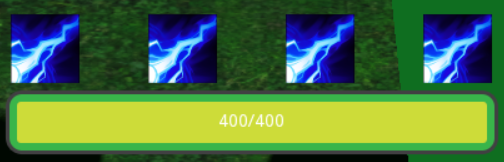
\includegraphics[width=0.8\linewidth]{figures/PlayerHUD}
	\caption{Habilidades del personaje y barra de vida.}
	\label{fig:PlayerHUD}
\end{figure}

\subsubsection{Match details}
En esta sección se muestra el estado actual de los objetivos de la partida. La información mostrada variará según el modo del juego, estos son:
\begin{itemize}
	\item \textbf{Deathmatch}: Se mostrará el número de vidas restantes de cada equipo.
	\item \textbf{Captura}: Se mostrará la puntuación de cada equipo así como el tiempo de partida restante (ver figura \ref{fig:MatchDetails}).
\end{itemize}

\begin{figure}[h]
	\centering
	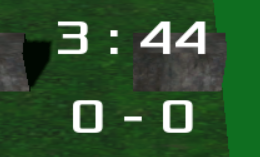
\includegraphics[width=0.8\linewidth]{figures/MatchDetails}
	\caption{Match Details del modo de juego \emph{Captura}.}
	\label{fig:MatchDetails}
\end{figure}

\subsection{Chat}
El juego tendrá dos chats: lobby y in-game. En la versión actual del juego, no hemos implementado todavía ninguno de ellos.

\vspace{\baselineskip}

El chat del lobby se podrá usar, antes de elegir equipo, para hablar con los otros tres jugadores (por ejemplo, para intentar "reclutar" a otro jugador con el que quieres jugar, antes de realizar la votación). Una vez que se ha votado y formado los dos equipos, se podrá usar el chat durante la fase de mejora de habilidades, pero solo para hablar con el compañero de equipo.

El chat in-game se podrá usar para hablar con el compañero de equipo durante toda la partida. Así, se proporciona al jugador una vía de comunicación para facilitar la cooperación.

\subsection{Menús}

\subsubsection{Menú principal}
El menú principal es lo primero que ve el jugador al entrar en el juego. Muestra la información del usuario (nombre, nivel y cantidad de monedas del juego de las que dispone (aunque todavía no hemos implementado nada de esto)) y diversos botones que permiten:

\begin{itemize}
	\item Ver el historial de partidas jugadas recientemente (no implementado). 
	\item Ver el puesto en la escalera clasificatoria (no implementado).
	\item Acceder a la configuración del juego (controles, audio y sonido). Por ahora, solo hemos implementado el menú de sonido (ver \emph{Menú de Sonido})
	\item Ver los amigos conectados (no implementado). El jugador puede agregar a otros jugadores dentro del juego para tenerlos en la lista de amigos y poder hablar con ellos. En el futuro, pensaremos en introducir algún modo de juego donde se pueda elegir jugar con/contra amigos.
	\item Acceder a la tienda del juego (no implementado). Aquí podrá comprar nuevos personajes, cosméticos, etc.
	\item Ver la información de los personajes (ver \emph{Menú de Personajes}).
	\item Buscar partida (al pulsar el botón \emph{Search Game}).
\end{itemize}

\begin{figure}[h]
	\centering
	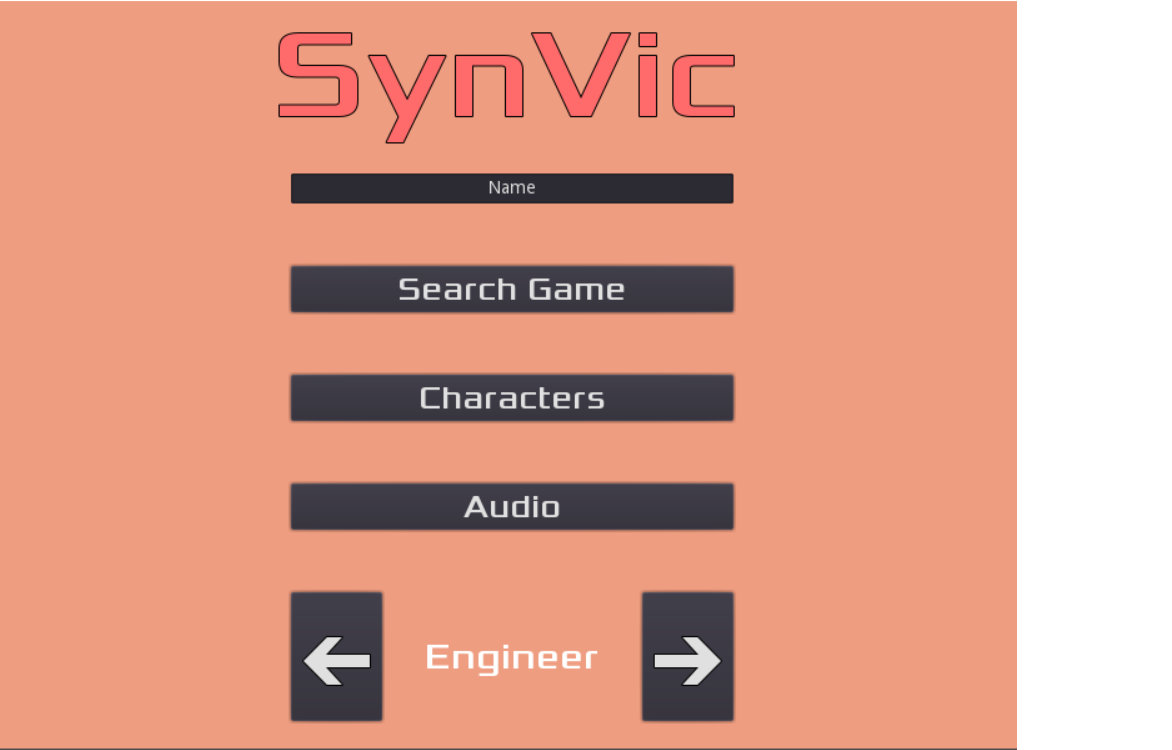
\includegraphics[width=0.7\linewidth]{figures/MainMenu}
	\caption{Menú principal del juego.}
	\label{fig:MainMenu}
\end{figure}

\subsubsection{Menú de Sonido}
Este menú permite al usuario configurar de forma separada el volumen maestro (que afecta a todo el sonido del juego), el volumen de la música y el volumen de los efectos de sonido. Además, se puede directamente silenciar cada uno de estos volúmenes por separado.

\begin{figure}[h!]
	\centering
	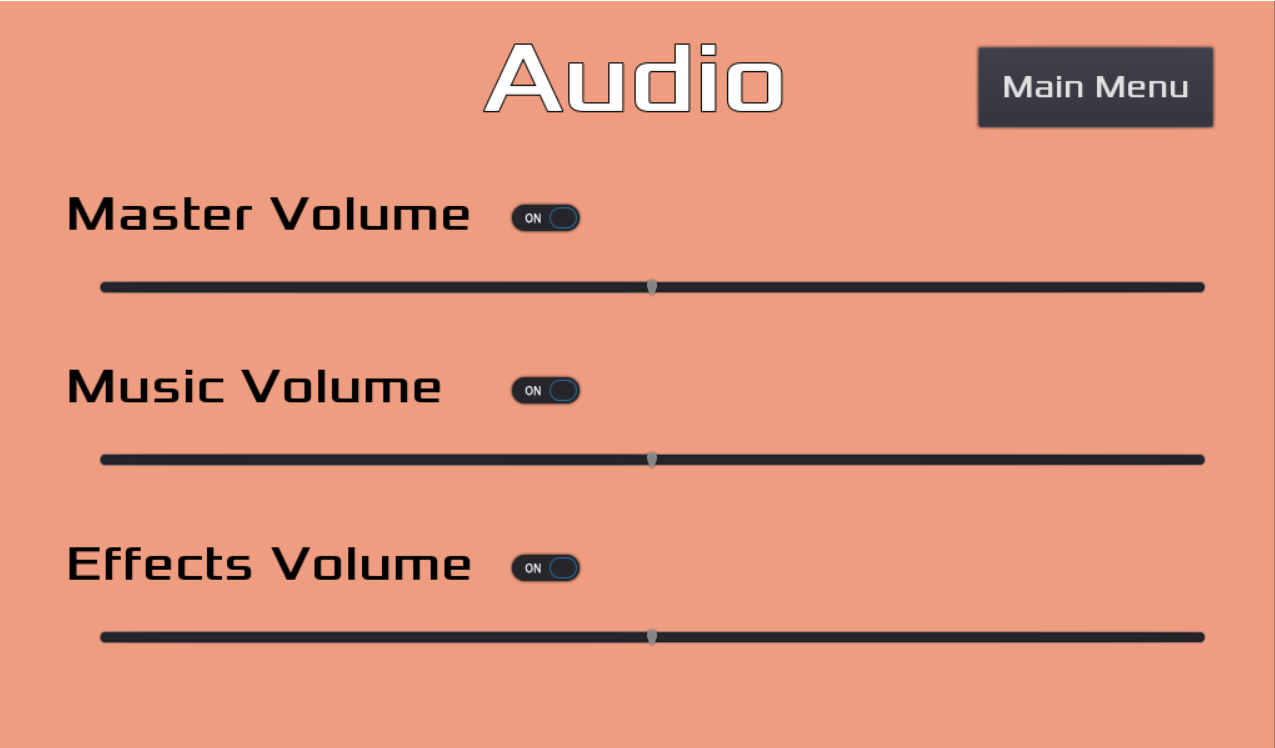
\includegraphics[width=0.7\linewidth]{figures/AudioMenu}
	\caption{Menú de configuración de sonido.}
	\label{fig:AudioMenu2}
\end{figure}

\subsubsection{Menú de Personajes}
En este menú, el jugador puede acceder a la información sobre cualquier personaje, incluyendo el funcionamiento de sus habilidades. De esta forma, el jugador puede informarse sobre lo que hace un personaje antes de jugar con él por primera vez.

\begin{figure}[h!]
	\centering
	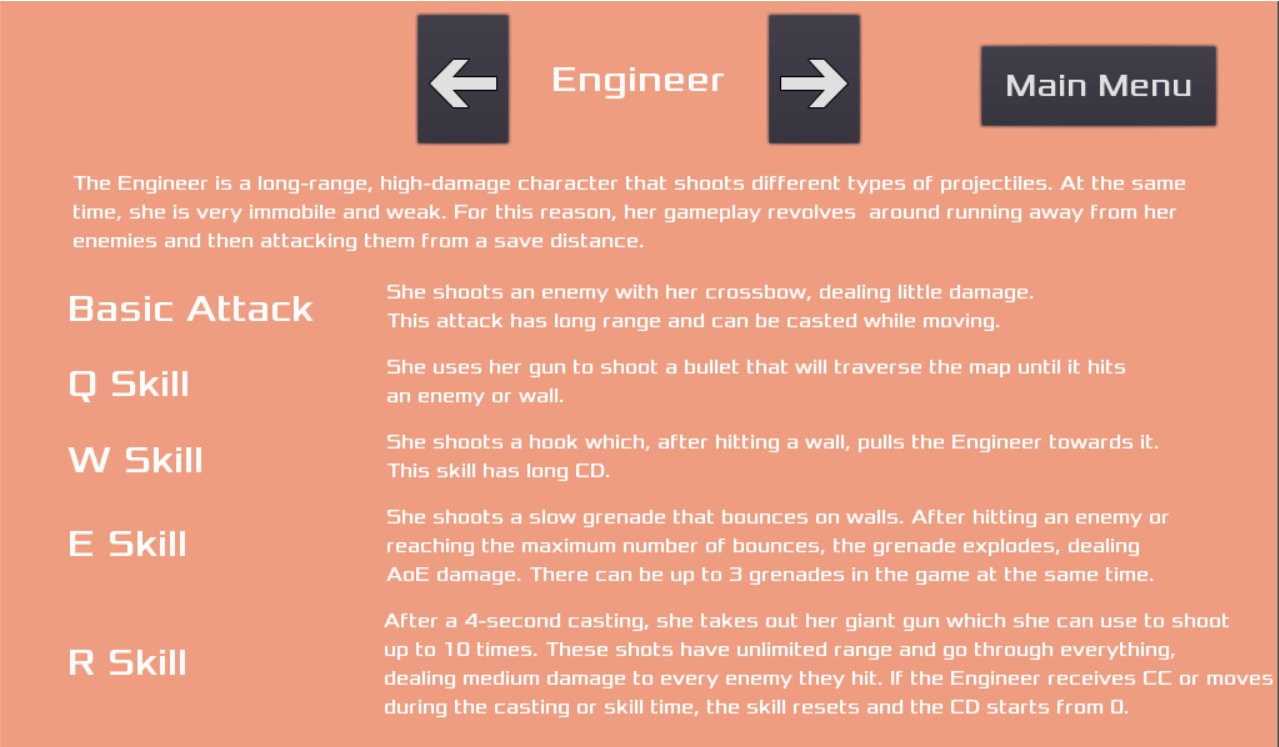
\includegraphics[width=0.7\linewidth]{figures/CharacterMenu}
	\caption{Menú de personajes.}
	\label{fig:CharacterMenu}
\end{figure}


\subsubsection{Lobby}
Tras encontrar una partida, el jugador accede al lobby junto a otros tres jugadores. Aquí, primero tendrá que votar para elegir a su compañero de equipo y, tras formar los equipos, elegir qué habilidades de su personaje mejorar (esto último todavía no está implementado).

\begin{figure}[h!]
	\centering
	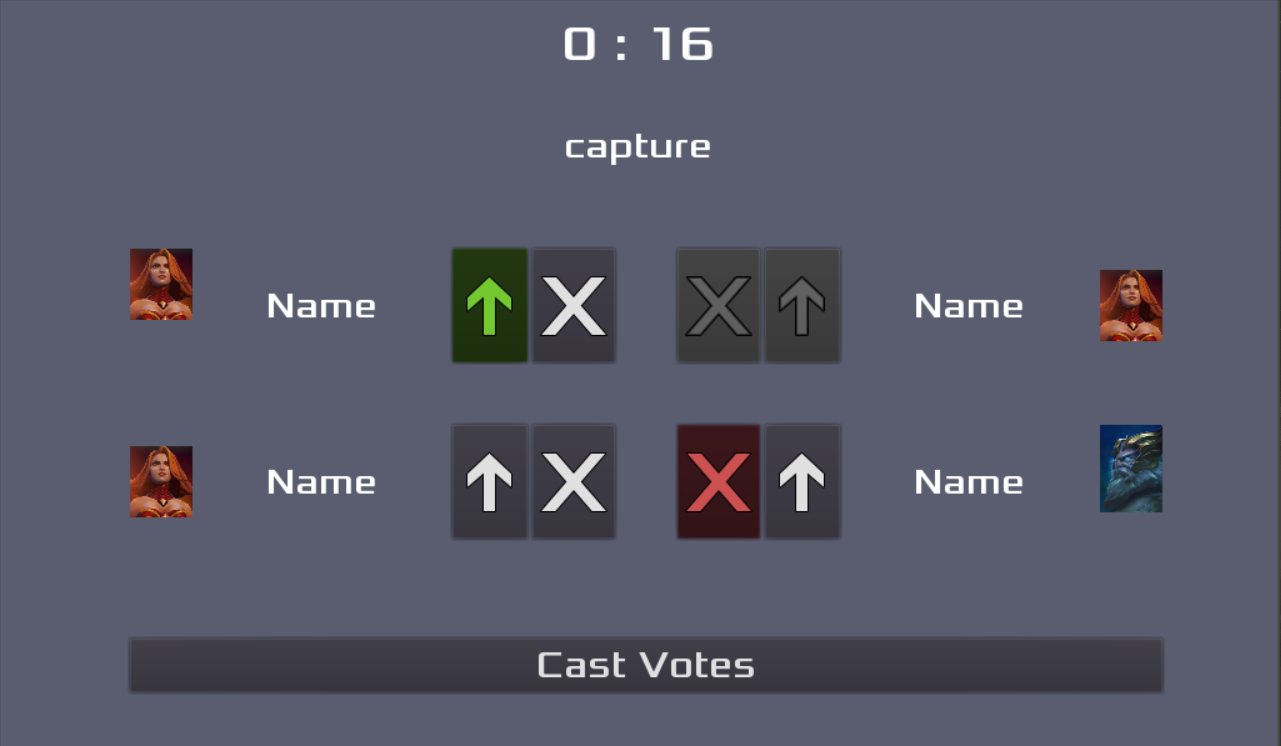
\includegraphics[width=0.7\linewidth]{figures/Lobby}
	\caption{Lobby.}
	\label{fig:Lobby}
\end{figure}

% ==============================================================================

\section{Sistema de control}
El juego usa un sistema de control por teclado y ratón. El usuario puede mover y rotar al personaje mediante clicks derechos del ratón. Si cliquea sobre un enemigo, el personaje aplicará un ataque básico sobre este.
Las teclas Q W E sirven para activar las tres habilidades básicas y la tecla R para la habilidad especial.

\vspace{\baselineskip}

La cámara del jugador tiene dos modos: \emph{auto} y \emph{manual}. En modo \emph{auto}, la cámara sigue el movimiento del jugador y siempre está centrada sobre este. En modo \emph{manual}, la cámara está fija y no sigue al jugador. En este modo, es el jugador el que debe mover la cámara arrastrando el ratón hacia los bordes de la pantalla. Al pulsar la tecla \emph{Space}, se cambia entre un modo y otro.